\section{Técnicas de Deep Learning y métodos de evaluación}
\label{sec:tecnicas_de_deep_learning_y_metodos_de_evaluacion}

\subsection{Técnicas de Deep Learning a utilizar en el proyecto}

A continuación se explicarán las principales técnicas utilizadas para el desarrollo del proyecto. Algunas de las técnicas que se mencionan no son específicas del deep learning.

\subsubsection*{\textit{Hold-out}}

El entrenamiento de las redes neuronales YOLO se ha realizado siguiendo esta técnica. Hold-out no es una técnica específica del deep learning, sino que es una técnica general que aplica sobre cualquier algoritmo de aprendizaje. Consiste en dividir el conjunto de datos en dos subconjuntos: uno que se utiliza para el entrenamiento y otro que únicamente se utiliza para evaluar el modelo obtenido tras el entrenamiento.

\subsubsection*{\textit{Red Neuronal Convolucional (CNN)}}

Tal y como se ha comentado en el tema \textit{\ref{sec:estado_del_arte} - \nameref{sec:estado_del_arte}}, YOLO es una red neuronal convolucional, por lo que antes de entrar en los detalles se va a explicar cómo funciona una CNN \cite{s5_cnn1} \cite{s5_cnn2}.

Las CNNs están compuestas por una sucesión de capas convolucionales, para la extracción de características, seguidas de unas capas perceptrón simples, para la clasificación final. Las capas convolucionales forman una jerarquía, de forma que las capas del principio son capaces de detectar formas básicas y cuanto más ``profunda'' es la capa, más complejas son las formas que son capaces de detectar. Por ejemplo: una capa inicial sería capaz de detectar líneas y círculos, mientras que una capa profunda sería capaz de detectar una cara.

Cada capa convolucional recibe como entrada una matriz bidimensional. En el caso de tratarse de la primera capa la entrada se corresponde directamente con la imagen, si se trata de una capa más profunda la entrada se corresponde con la salida de la capa anterior. Además, cada capa tiene definido un \textit{kernel}, que no es más que otra matriz bidimensional de dimensiones reducidas. Con la matriz de entrada y el kernel se realiza la operación de \textit{convolución}.

\begin{figure}[H]
	\centering
	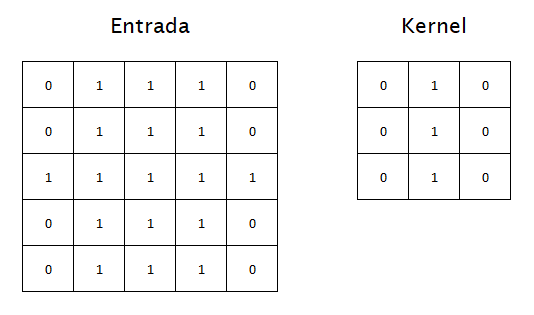
\includegraphics[width=0.7\linewidth]{images/convolutional_neuron_example.png}
	\caption{Ejemplo de capa convolucional con una entrada de 5x5 y un kernel de 3x3}
	\label{fig:cnn_neuronex}
\end{figure}

La operación de \textit{convolución} consiste en hacer un barrido del \textit{kernel} por la matriz de entrada, de izquierda a derecha y de arriba a abajo. En cada una de las posiciones del barrido se aplica el producto escalar entre el kernel y la submatriz de la matriz de entrada sobre la que se encuentre. En la figura \ref{fig:cnn_convolutionoperationex} se puede ver gráficamente el proceso.

\begin{figure}[H]
	\centering
	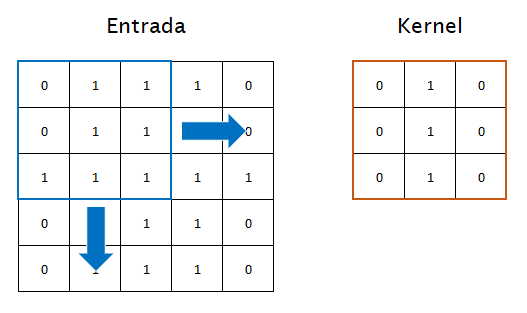
\includegraphics[width=0.7\linewidth]{images/convolutional_operation_example.png}
	\caption{Representación gráfica de operación convolucional}
	\label{fig:cnn_convolutionoperationex}
\end{figure}

Para realizar el producto escalar, las matrices se \textit{aplanan}, de tal forma que la submatriz de entrada quedaría de la siguiente forma:

\begin{equation}
	\left[
	\begin{array}{ccc}
		0 & 1 & 1 \\
		0 & 1 & 1 \\
		0 & 1 & 1 \\
	\end{array}
	\right]
	=>
	\left[
	\begin{array}{ccccccccc}
		0 & 1 & 1 & 0 & 1 & 1 & 0 & 1 & 1 \\
	\end{array}
	\right]
	\nonumber
\end{equation}

El kernel:

\begin{equation}
	\left[
	\begin{array}{ccc}
		0 & 1 & 0 \\
		0 & 1 & 0 \\
		0 & 1 & 0 \\
	\end{array}
	\right]
	=>
	\left[
	\begin{array}{ccccccccc}
		0 & 1 & 0 & 0 & 1 & 0 & 0 & 1 & 0 \\
	\end{array}
	\right]
	\nonumber
\end{equation}

Y por lo tanto el producto escalar:

\begin{equation}
	\left[
	\begin{array}{ccccccccc}
		0 & 1 & 1 & 0 & 1 & 1 & 0 & 1 & 1 \\
	\end{array}
	\right]
	\left[
	\begin{array}{c}
		0 \\
		1 \\
		0 \\
		0 \\
		1 \\
		0 \\
		0 \\
		1 \\
		0 \\
	\end{array}
	\right] = 3
	\nonumber
\end{equation}

Como resultado de aplicar la convolución sobre la matriz de entrada se obtiene una nueva matriz. Además del kernel, las capas convolucionales tienen otros parámetros asociados, como por ejemplo, cómo de rápido avanza el kernel durante el barrido.

Las capas convolucionales no tiene un único kernel asociado, sino que tienen varios. Teniendo en cuenta esto y suponiendo que tenemos como entrada una imagen en blanco y negro de $28x28x1$ píxeles y que cada capa tiene $32$ kernels de $3x3$, la primera capa convolucional estaría compuesta por $28 x 28 = 784$ neuronas, y tras aplicar la operación de convolución, se obtendrían como resultado $32$ nuevas matrices de dimensiones $26 x 26$, que harían necesarias $26 x 26 x 32 = 21.632$ neuronas en la segunda capa. Teniendo en cuenta que una CNN puede estar compuesta por varias decenas de capas, se hace necesario introducir un mecanismo de reducción, para que el número de neuronas necesarias no crezca tan desmesuradamente con cada capa. Este mecanismo se conoce como \textit{pooling}. El \textit{MaxPooling}, es un tipo de pooling comunmente usado, y consiste en deslizar una ventana bidimensional sobre la matriz de entrada, de izquierda a derecha y de arriba a abajo. En cada una de las posiciones se tomará como valor resultante el máximo valor presente en la ventana. La capacidad de reducción del MaxPooling depende de dos factores: el tamaño de la ventana y el tamaño del salto que se da hacia la derecha y hacia abajo. En la figura \ref{fig:cnn_maxpooling} se muestra un ejemplo gráfico.

\begin{figure}[H]
	\centering
	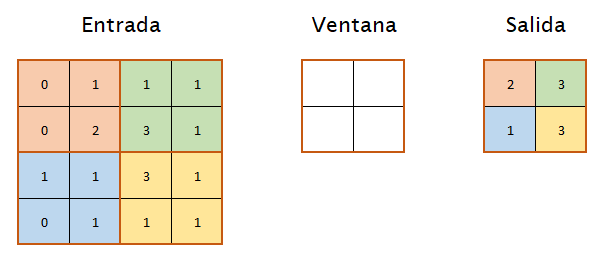
\includegraphics[width=0.7\linewidth]{images/maxpooling_example.png}
	\caption{Representación gráfica de MaxPooling con una entrada de 4x4, una ventana de 2x2 y un salto de 2}
	\label{fig:cnn_maxpooling}
\end{figure}

\subsubsection*{Transferencia de conocimiento (transfer learning)}

% Otra de las técnicas que se han utilizado en el proyecto es la denominada \textit{transferencia del conocimiento (transfer learning)}.

Entrenar un modelo de detección de objetos es un proceso muy costoso, ya que se necesita un gran volumen de imágenes y una gran capacidad de cómputo. El \textit{transfer learning} viene a paliar este problema ya que permite utilizar un modelo ya entrenado como punto de partida para entrenar otro. Como se ha comentado anteriormente, las primeras capas de una CNN son capaces de detectar formas básicas y a medida que se profundiza en las capas, estas detectan formas más específicas. Si ya tenemos entrenado un modelo \texttt{X} para detectar un determinado tipo de objetos y queremos entrenar otro \texttt{Y} para detectar otro tipo de objetos, las primeras capas de ambos modelos van a detectar el mismo tipo de formas, y serán las capas más profundas las que se diferencien. Por lo tanto podríamos utilizar el modelo \texttt{X} como punto de partida para el modelo \texttt{Y}, y este último podrá beneficiarse del conocimiento transferido aprender más rápido.

Esta técnica se ha utilizado ampliamente durante la fase de entrenamiento. Se ha utilizado para aprovechar el conocimiento de los modelos YOLO ya entrenados proporcionados por sus autores. También se ha utilizado para lidiar con las limitaciones de uso que tiene la infraestructura utilizada durante el entrenamiento.

\subsubsection*{YOLO V3}

En la figura \ref{fig:yolov3architecture} se muestra la arquitectura de YOLO V3 de tamaño 416x416. Está compuesta por un total de 106 capas convolucionales. Tiene una única entrada, de dimensiones 416x416x3, y tres salidas de dimensiones 13x13x255, 26x26x255 y 52x52x255 respectivamente. Las tres salidas se corresponden con 3 escalas de detección de objetos, la primera de ellas sirve para detectar objetos grandes, la segunda objetos medianos y la tercera objetos pequeños.

Como se explicó en el tema \textit{\ref{sec:estado_del_arte} - \nameref{sec:estado_del_arte}}, YOLO divide la imagen en una rejilla de $SxS$ celdas. En realidad, divide la imagen en tres rejillas que se corresponden con las 3 salidas. Para cada una de las celdas de estas rejillas se proponen un número $B$ regiones candidatas, en este caso son 5. Cada una de estas regiones candidatas están representadas por 5 variables, 4 para la región propiamente dicha y 1 para indicar la probabilidad de que la región contenga un objeto. YOLO es capaz de detectar 80 clases de objetos, por lo que junto a cada región candidata se añaden otras 80 variables para indicar la probabilidad de pertenencia a cada una de las clases. Con todo esto, cada una de las celdas de las rejillas se compone de $3 x (5 + 80) = 255$ variables.

\begin{figure}[H]
	\centering
	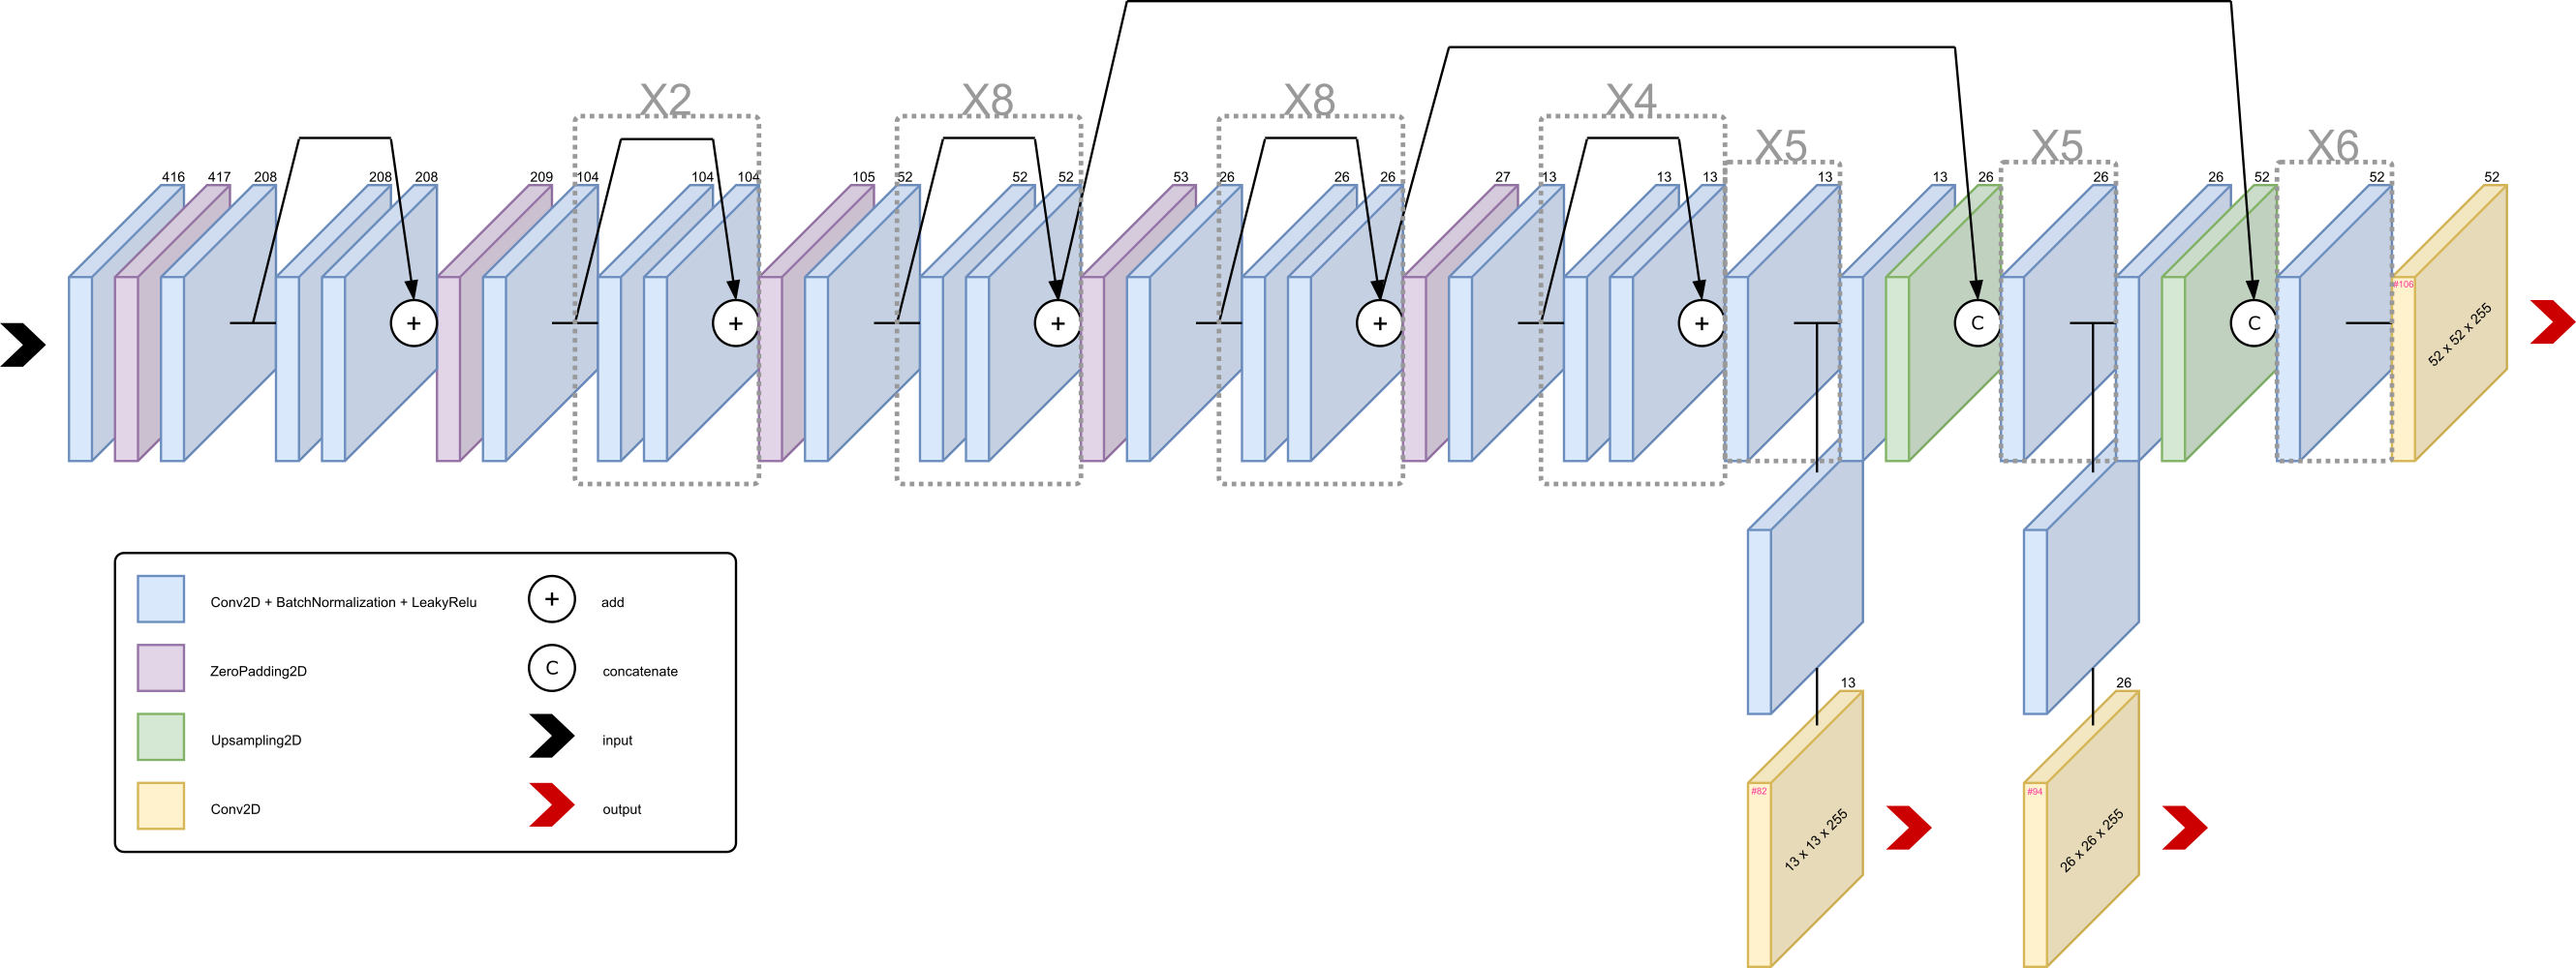
\includegraphics[width=\linewidth]{images/yolo_v3_architecture.png}
	\caption{Arquitectura de YOLO V3 de tamaño 416x416}
	\label{fig:yolov3architecture}
\end{figure}

\subsubsection*{YOLO V3 Tiny}

En la figura \ref{fig:yolov3tinyarchitecture} se muestra la arquitectura YOLO V3 Tiny de tamaño 416x416. Está compuesta por un total de 13 capas convolucionales. Tiene una única entrada, de dimensiones 416x416, y dos salidas de dimensiones 13x13x255 y 26x26x255 respectivamente. El fundamento es el mismo que en YOLO V3. Se han reducido el número de capas convolucionales de manera considerable, lo cual simplifica el modelo y hace que sea apto para ejecutarse en un dispositivo con recursos limitados manteniendo la premisa de ser capaz de detectar objetos en tiempo real.

\begin{figure}[H]
	\centering
	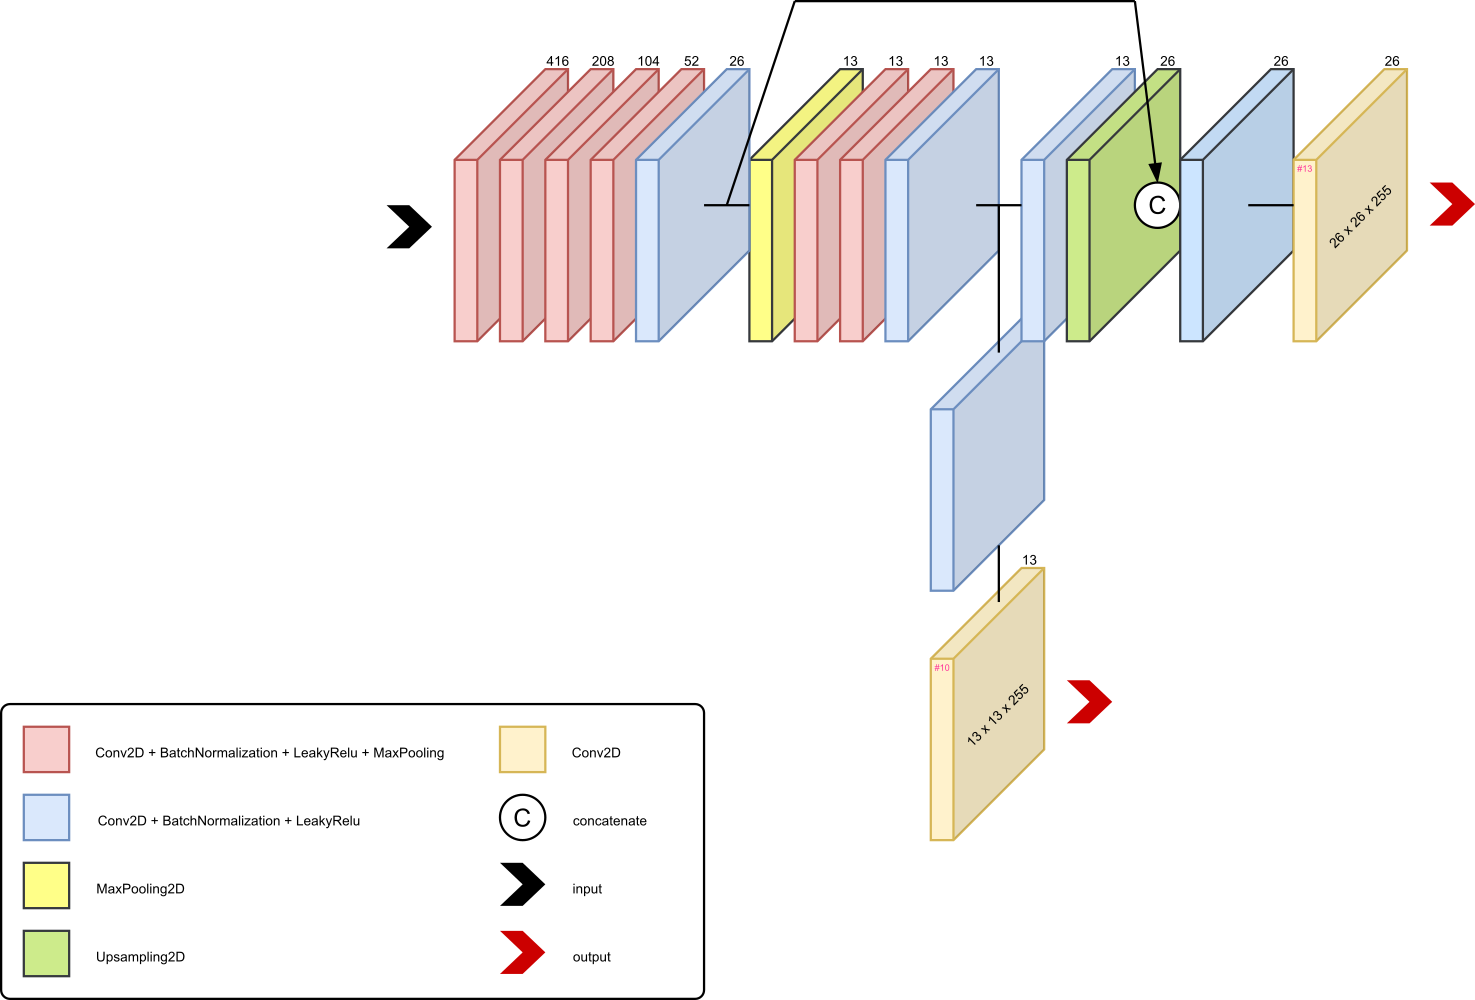
\includegraphics[width=\linewidth]{images/yolo_v3_tiny_architecture.png}
	\caption{Arquitectura de YOLO V3 Tiny de tamaño 416x416}
	\label{fig:yolov3tinyarchitecture}
\end{figure}

\subsection{Métodos de evaluación a utilizar en el proyecto}

La métrica que se ha utilizado para evaluar los modelo obtenidos es la \textbf{AP (Average Precision)}, que es la métrica que se utiliza en los problemas de detección de objetos.

Antes de explicar en qué consiste la métrica AP hay que explicar una serie de conceptos en los cuales está basada: \textbf{IoU (intersección sobre la unión)}, \textbf{precisión (precision)} y \textbf{sensibilidad (recall)}.

El concepto de \textit{IoU} mide cuánto se solapan dos regiones: la predicha y la que debería ser detectada. Se calcula dividiendo la región obtenida mediante la intersección de la región predicha y la región a detectar entre la región obtenida mediante la unión de ambas regiones.

\begin{equation}
	AP = \frac{interseci\acute{o}n}{uni\acute{o}n} = \frac{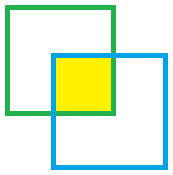
\includegraphics[width=0.2\linewidth]{images/ap_intersection.png}}{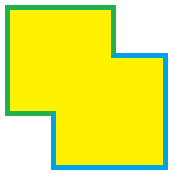
\includegraphics[width=0.2\linewidth]{images/ap_union.png}}
	\nonumber
\end{equation}

La \textit{precisión} (precision) mide la capacidad del modelo para detectar únicamente los objetos relevantes. Se calcula como el porcentaje de predicciones positivas acertadas frente a todas las predicciones positivas predichas:

\begin{equation}
	precisi\acute{o}n = \frac{TP}{TP + FP} = \frac{TP}{todas\ las\ predicciones\ positivas}
	\nonumber
\end{equation}

La \textit{sensibilidad} (recall)  mide la capacidad del modelo para detectar todos los objetos relevantes. Se calcula como el porcentaje de predicciones positivas acertadas frente a todas las existentes:

\begin{equation}
	sensibilidad = \frac{TP}{TP + FN} = \frac{TP}{todas\ las\ regiones\ a\ detectar}
	\nonumber
\end{equation}

Tanto en el cálculo de la \textit{precisión} como en de la \textit{sensibilidad}, para determinar si una predicción es positiva, se utiliza el \textit{IoU}. Se define un umbral para el \textit{IoU} (normalmente suele ser 0.5) y si se supera dicho umbral, la predicción es considerada positiva.

La métrica \textit{AP} se calcula como el área debajo de la \textbf{curva precisión-sensibilidad} (precision-recall). En el eje de las abscisas se representa la \textit{sensibilidad} (recall) y en el eje de las ordenadas se representa la \textit{precisión} (precision).

A continuación se va a mostrar un ejemplo práctico de cómo se calcula la \textit{AP}. Para este ejemplo se dispone de una serie de imágenes con un total de 4 baches a detectar. En la tabla \ref{tab:apprecisionrecalltable} se puede ver el cálculo de la \textit{precisión} y de la \textit{sensibilidad} para las predicciones obtenidas. La columna \textit{Positivo} indica si la predicción es positiva, es decir, si el valor de \textit{IoU} supera el umbral definido, que en este caso es 0.5. Las columnas \textit{TP} y \textit{FP} muestran el acumulado de sus respectivos valores.

\begin{table}[H]
	\centering
	\begin{tabular}{rrrrrr}
		\toprule
		IoU &  Positivo &  TP &  FP &  Precisión &  Sensibilidad \\
		\midrule
		0.912933 &         1 &   1 &   0 &   1.000000 &          0.25 \\
		0.711111 &         1 &   2 &   0 &   1.000000 &          0.50 \\
		0.387983 &         0 &   2 &   1 &   0.666667 &          0.50 \\
		0.387983 &         0 &   2 &   2 &   0.500000 &          0.50 \\
		0.387983 &         0 &   2 &   3 &   0.400000 &          0.50 \\
		1.000000 &         1 &   3 &   3 &   0.500000 &          0.75 \\
		0.225986 &         0 &   3 &   4 &   0.428571 &          0.75 \\
		0.225986 &         0 &   3 &   5 &   0.375000 &          0.75 \\
		1.000000 &         1 &   4 &   5 &   0.444444 &          1.00 \\
		\bottomrule
	\end{tabular}
	\caption{Cálculo de la precisión y sensibilidad para las predicciones}
	\label{tab:apprecisionrecalltable}
\end{table}

Una vez se tienen calculados los valores de \textit{precisión} y de \textit{sensibilidad} se calcula la curva \textit{precisión-sensibilidad} como se puede ver en la figura \ref{fig:apprecisionrecallcurve}. Para realizar el cálculo del área debajo de la curva se realiza un suavizado de la misma. Este suavizado consiste en establecer como valor de \textit{precisión} para un determinado valor de \textit{sensibilidad}, el valor de \textit{precisión} más alto que se encuentre a su derecha. Por ejemplo, para la \textit{sensibilidad} 0.6 se establece como valor de \textit{precisión} el valor más alto a su derecha, que en este caso es 0.5. En color naranja se puede ver la curva suavizada.

\begin{figure}[H]
	\centering
	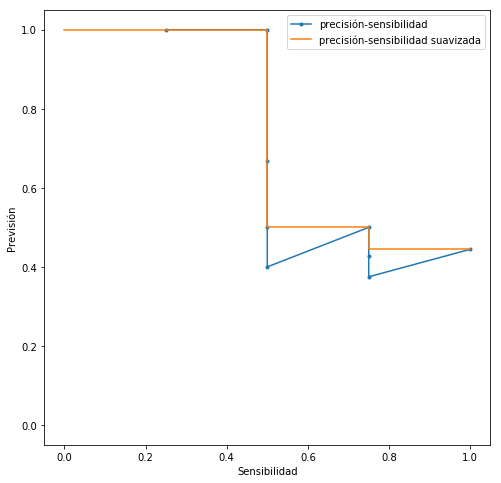
\includegraphics[width=0.7\linewidth]{images/ap_precision_recall_curve.png}
	\caption{Curva precisión-sensibilidad}
	\label{fig:apprecisionrecallcurve}
\end{figure}

Por lo que finalmente, para este ejemplo, el cálculo del \textit{AP} sería:

\begin{equation}
	AP = (0.5 - 0) \cdot 1 + (0.75 - 0.5) \cdot 0.5 + (1 - 0.75) \cdot 0.44 = 0.5 + 0.125 + 0.11 = \textbf{0.735}
	\nonumber
\end{equation}